% ---------- Titelblad Masterproef Faculteit Wetenschappen -----------
% Dit document is opgesteld voor compilatie met pdflatex.  Indien je
% wilt compileren met latex naar dvi/ps, dien je de figuren naar
% (e)ps-formaat om te zetten.
%                           -- december 2012
% -------------------------------------------------------------------
\RequirePackage{fix-cm}
\documentclass[12pt,a4paper,oneside]{book}

% --------------------- In te laden pakketten -----------------------
% Deze kan je eventueel toevoegen aan de pakketten die je al inlaadt
% als je dit titelblad integreert met de rest van thesis.
% -------------------------------------------------------------------
\usepackage{graphicx,xcolor,textpos}
\usepackage{helvet}
\usepackage[linktoc=all]{hyperref}
\usepackage[dutch]{babel}
\usepackage{slashbox}

\graphicspath{{images/}}

% -------------------- Pagina-instellingen --------------------------
% Indien je deze wijzigt, zal het titelblad ook wijzigen.  Dit dien je
% dan manueel aan te passen.
% --------------------------------------------------------------------

\topmargin -10mm
\textwidth 160truemm
\textheight 240truemm
\oddsidemargin 0mm
\evensidemargin 0mm

% ------------------- textpos-instellingen ---------------------------
% Enkele andere instellingen voor het voorblad.
% --------------------------------------------------------------------

\definecolor{green}{RGB}{172,196,0}
\definecolor{bluetitle}{RGB}{29,141,176}
\definecolor{blueaff}{RGB}{0,0,128}
\definecolor{blueline}{RGB}{82,189,236}
\setlength{\TPHorizModule}{1mm}
\setlength{\TPVertModule}{1mm}

\begin{document}

% ---------------------- Voorblad ------------------------------------
% Vergeet niet de tekst aan te passen:
% - Titel en, indien van toepassing, ondertitel
%          voor eventuele formules in de titel of ondertitel
%          gebruik je  \form{$...$}
% - Je naam
% - Je (co)promotor, begeleider (indien van toepassing)
% - Je opleiding
% - Het academiejaar
% --------------------------------------------------------------------
\thispagestyle{empty}
\newcommand{\form}[1]{\scalebox{1.087}{\boldmath{#1}}}
\sffamily
%
\begin{textblock}{191}(-24,-11)
\colorbox{green}{\hspace{123mm}\ \parbox[c][18truemm]{68mm}{\textcolor{white}{FACULTEIT WETENSCHAPPEN}}}
\end{textblock}
%
\begin{textblock}{70}(-18,-19)
\textblockcolour{}
\includegraphics*[height=19.8truemm]{LogoKULeuven}
\end{textblock}
%
\begin{textblock}{160}(-6,63)
\textblockcolour{}
\vspace{-\parskip}
\flushleft
\fontsize{40}{42}\selectfont \textcolor{bluetitle}{Programmeren met Onzekerheid: Een Case Study}\\[1.5mm]
\fontsize{20}{22}\selectfont Ondertitel \form{$S=\pi r^2$\textsl{(facultatief)}}
\end{textblock}
%
\begin{textblock}{160}(8,153)
\textblockcolour{}
\vspace{-\parskip}
\flushright
\fontsize{14}{16}\selectfont \textbf{Sus VERWIMP}
\end{textblock}
%
\begin{textblock}{70}(-6,191)
\textblockcolour{}
\vspace{-\parskip}
\flushleft
Promotor: Prof. T. Schrijvers\\[-2pt]
\textcolor{blueaff}{Affiliatie \textsl{(facultatief)}}\\[5pt]
%Co-promotor: \textsl{(facultatief)}\\[-2pt]
%\textcolor{blueaff}{Affiliatie \textsl{(facultatief)}}\\[5pt]
Begeleider: \textsl{A. Vandenbroucke (facultatief)}\\[-2pt]
\textcolor{blueaff}{Affiliatie \textsl{(facultatief)}}\\
\end{textblock}
%
\begin{textblock}{160}(8,191)
\textblockcolour{}
\vspace{-\parskip}
\flushright
Proefschrift ingediend tot het\\[4.5pt]
behalen van de graad van\\[4.5pt]
Master of Science in\\[4.5pt]
Toegepaste Informatica\\
\end{textblock}
%
\begin{textblock}{160}(8,232)
\textblockcolour{}
\vspace{-\parskip}
\flushright
Academiejaar 2017-2018
\end{textblock}
%
\begin{textblock}{191}(-24,248)
{\color{blueline}\rule{550pt}{5.5pt}}
\end{textblock}
%
\vfill
\newpage
\thispagestyle{empty}
% Copyright statement
\textsf{\textcopyright} Copyright by KU Leuven
Zonder voorafgaande schriftelijke toestemming van zowel de promotor(en) als de auteur(s) is overnemen, kopiëren, gebruiken of realiseren van deze uitgave of gedeelten ervan verboden. Voor aanvragen tot of informatie i.v.m. het overnemen en/of gebruik en/of realisatie van gedeelten uit deze publicatie, wend u tot de KU Leuven, Faculteit Wetenschappen, Geel Huis, Kasteelpark Arenberg 11 bus 2100, 3001 Leuven (Heverlee), Telefoon +32 16 32 14 01.
\\\\
Voorafgaande schriftelijke toestemming van de promotor(en) is eveneens vereist voor het aanwenden van de in dit afstudeerwerk beschreven (originele) methoden, producten, schakelingen en programma’s voor industrieel of commercieel nut en voor de inzending van deze publicatie ter deelname aan wetenschappelijke prijzen of wedstrijden.

\vfill
\newpage

% Als je het titelblad wil integreren met de rest van je thesis,
% kan je hieronder verder.
% ----------------------- Eerste pagina's -------------------------
% Hier kan je inhoudsopgave, voorwoord en dergelijke kwijt.
% -----------------------------------------------------------------
\rmfamily
\setcounter{page}{0}
\pagenumbering{roman}
\frontmatter
\chapter{Voorwoord}
\chapter{Korte Samenvatting}
\chapter{Lijst van afkortingen en lijst van symbolen}
\tableofcontents


\newpage
% ----------------------- Eigenlijke thesis -----------------------
% Vanaf de inleiding/het eerste hoofdstuk.
% -----------------------------------------------------------------
\mainmatter
\setcounter{page}{0}
\pagenumbering{arabic}

\chapter{Inleiding}
De grote interesse in het domein ‘onzekerheid’ in AI resulteert in de ontwikkeling van verschillende programmeertalen. Deze talen worden probabilistische programmeertalen of PPL (Probabilistic Programming Language) genoemd. Een PPL heeft in grote lijnen 2 hoofdfuncties:
\begin{itemize}
  \item Het modelleren van een wereld met onzekerheid
  \item Het redeneren/infereren van vragen over deze wereld
\end{itemize}
Voorheen was het zeer moeilijk als programmeur om werelden met onzekerheid te modelleren, laat staan het redeneren over deze werelden. Met de komst van PPL’s is dit probleem al een stuk makkelijker geworden.
Elke PPL heeft zijn eigen manier van implementatie en wordt vaak geïmplementeerd als extensie op een general-purpose programmeertaal. Dit zorgt ervoor dat de PPL niet gelimiteerd is aan een kleine subset van de werelden die het kan modelleren. Veel van deze PPL’s streven naar een balans tussen performantie en expressiviteit. Het is belangrijk voor een PPL om genoeg werelden te kunnen simuleren en op een aanneembare tijd te kunnen redeneren over vragen over deze wereld.
\\\\
Omdat er zo veel PPL’s beschikbaar zijn de laatste jaren is het niet altijd duidelijk welke voordelen of nadelen ze hebben ten opzichte van andere PPL’s. Verschillende van deze PPL’s zijn in recente artikels vergeleken met elkaar aan de hand van eigenschappen en concepten van de taal (Probabilistic (Logic) Programming Concepts, Luc De Raedt - Angelika Kimmig). Andere artikels vergelijken PPL’s aan de hand van hun vorige iteratie of PPL’s met hetzelfde programmeerparadigma (Inference and Learning in Probabilistic Logic Programs using Weighted Boolean Formulas, LUC DE RAEDT et al). Deze artikels evalueren PPL’s met hetzelfde programmeerparadigma zoals logische probabilistische programmeertalen of functionele probabilistische programmeertalen.
\\\\
In deze thesis ben ik van plan PPL’s met verschillende programmeerparadigma zoals ProbLog en Anglican te evalueren. ik ga deze PPL’s evalueren ten opzichte van elkaar aan de hand van qualitatieve en quantitatieve criteria zoals: performantie, expressiviteit, geheugengebruik, uitbreidbaarheid, tools beschikbaar, moeilijkheidsgraag,... Omdat het niet triviaal is om programmeertalen te vergelijken die totaal anders geïmplementeerd zijn maak ik gebruik van een case study. Ik begin met het verzinnen van een onzekerheidsprobleem waarna ik uitleg geef waarom ik gekozen heb voor dit probleem. Daarna evalueer ik de implementatie van het probleem in de verschillende PPL’s aan de hand van vooropgestelde criteria. Ten slotte volgt een evaluatie van de PPL’s ten opzichte van elkaar. Uiteindelijk wil ik kunnen aantonen welke PPL het best presteert in welke criteria aan de hand van het opgegeven probleem.

\chapter{Achtergrond}
In deze sectie geef ik de nodige achtergrondinformatie om de rest van mijn thesis te begrijpen.
Onzekerheid in artificiele intelligentie is één van de invloedrijkste domeinen van artificiele intelligentie. De reden hiervoor is omdat de wereld van nature veel onzekerheid bevat. Denk aan de volgende punten:
\begin{itemize}
	\item Kennis (we kunnen niet alles van de wereld weten)
	\item Incomplete modellen (verschijnselen die niet onder het model vallen)
	\item Sensoren (we kunnen de wereld enkel observeren met de tools die beschikbaar zijn en deze zijn meestal nog foutgevoelig.)
	\item Acties (we kunnen niet elke actie uitvoeren)
\end{itemize}
Als we spreken over werken met onzekerheid bedoelen we het opstellen van een hypothese, en deze hypothese (zo goed mogelijk) bewijzen aan de hand van het gegeven bewijs van de wereld.
Er zijn 3 belangrijke kwesties in verband met het werken met onzekerheid:
\begin{itemize}
	\item Representeren van onzekerheid
	\item Redeneren over onzekerheid
	\item Leren aan de hand van onzekerheid
\end{itemize}
Het representeren van onzekerheid gebeurt in het model. Een model is een weergave van een onzekerheidsprobleem waarbij elke wereld kan gesimuleerd worden.
\\\\
Bij het redeneren over onzekerheid maken we gebruik van het model om vragen te stellen over mogelijke hypotheses. (vb. wat is de kans dat we een eerlijk muntstuk hebben als we deze 20 keer tossen en 15 keer hoofd en 5 keer munt verkrijgen). In dit voorbeeld is de hypothese “of het muntstuk eerlijk is”. Het bewijs dat we hebben is dat we 20 keer tossen en 15 keer hoofd en 5 keer munt kregen. Wat we willen is de kans dat de hypothese klopt, m.a.w. de kans dat het muntstuk eerlijk is.
\\\\\
Een manier om te berekenen wat de kans is of een munt eerlijk is, is het gebruik maken van de Bayes’s rule:
\begin{equation} 
	\label{eq:bayesrule}
	P(Hypothese|Bewijs) = \frac{P(Bewijs|Hypothese)P(Hypothese)}{P(Bewijs)}
\end{equation}
\\\\
Bayes' rule geeft de kans dat een hypothese waar is in een wereld waar er al dan niet bewijs is over deze wereld. Voor meer informatie verwijs ik naar het boek (Bayesian Reasoning and Machine Learning). PPL's kunnen hetzelfde berekenen aan de hand van een inferentie proces dat de taal implementeert. Elke PPL heeft een methode om de inferentie te bereken. Hoe ze dit doen verschilt voor elke PPL.
Het berekenen van de inferentie is een zeer krachtig, maar een zeer kostelijk proces qua rekenkracht. Veel PPL's zoeken een balans tussen hoe efficient ze inferentie kunnen berekenen en welke problemen ze kunnen modelleren (hoe expressief de taal is).
\\\\
Omdat het modelleren van een onzekerheidsprobleem, het redeneren over dit probleem en het leren aan de hand van de redeneringen een intensief proces is, is het beter om hiervoor computerkracht te gebruiken. Hierdoor werden er Probabilistische programmeertalen ontworpen.

\section{Probabilistische programmeertalen}
Probabilistische programmeertalen (of PPL's van Probabilistic Programming Languages) zijn programmeertalen met 2 hoofdfuncties:
\begin{itemize}
	\item Het modelleren van een wereld met onzekerheid
	\item Het redeneren/infereren van vragen over deze wereld
\end{itemize}
Er zijn PPL implementaties die een volledig nieuwe taal hebben geïmplementeerd speciaal voor het modelleren en redeneren, maar de meesten zijn geïmplementeerd als extensie op een bestaande general-purpose programmeertaal. In deze thesis maak ik gebruik van 2 PPL’s, namelijk: ProbLog2 en Anglican.
\subsection{ProbLog2}
ProbLog2 is een PPL die gebaseerd is op de Sato’s distribution semantics (Sato 1995). Het kan beschouwd worden als een Prolog programma met probabilistische aspecten geïmplementeerd. Een ProbLog programma bestaat uit feiten geannotteerd met kansen.
0.5 :: heads(C) :- coin(C).
coin(c1).
\\\\
In het bovenstaande voorbeeld hebben we 1 feit: coin(c1). en 1 probabilistisch predicaat: 0.5 :: heads(C) :- coin(C). wat dit programma zegt is dat het predicaat heads(C) waar is in de wereld met 50% kans voor elke munt die geïnstantieerd is als coin(C).
\\\\
We kunnen ook gebruik maken van “annotated disjunction” wat eigenlijk syntactische suiker is om hetzelfde te bereiken. Als we het vorige voorbeeld schrijven met “annotated disjunction” komen we tot:
0.5 :: heads(C, true); 0.5:: heads(C, false) :- coin(C).
coin(c1).
\\\\
In dit voorbeeld geeft het heads predicaat voor een bepaalde munt true voor 50% van de tijd en false voor 50% van de tijd. De totale kans voor het predicaat heads is 100%. Stel dat we heads(C,false). een kans geven van 0.4, dan hebben we 50% kans op true als parameter voor heads, 40% kans op false als parameter voor heads en 10% kans dat het predicaat zelf false terug geeft. Voor dit klein programma lijkt dit onnodig maar voor grotere probabilistische problemen kan “annotated disjunction” zeer handig zijn om een beter inzicht te krijgen over wat de probabilistische predicaten doen.
\\\\
De combinatie van deze regels en het logic programmeer systeem prolog geeft ons de mogelijkheid om zeer uitgebreide probabilistische werelden te modelleren. We kunnen vragen stellen aan deze modellen en aan de hand van de inferentie machine van ProbLog worden deze vragen opgelost.
\subsubsection{Inferentie}
Om vragen te stellen over het model maken we gebruik van queries en bewijzen. Als we willen berekenen hoeveel kans we hebben dat we 2 munten tossen en ze beiden op hoofd landen kunnen we dit doen aan de hand van het volgende programma:
0.5 :: heads1.
0.5 :: heads2.
two\textunderscore heads :- heads1, heads2.
query(two\textunderscore heads).
\\\\
Dit geeft het resultaat 0.25 wat uiteindelijk de kans is van ( ) ( ).
We kunnen het resultaat van de query manipuleren door bewijs te geven aan dit model. Stel dat we weten dat de eerste munt zeker hoofd als resultaat heeft, dan kunnen we dit als bewijs meegeven aan het model op de volgende manier:
0.5 :: heads1.
0.5 :: heads2.
two\textunderscore heads :- heads1, heads2.
Evidence(heads1, true).
query(two\textunderscore heads).
\\\\
Dit geeft het resultaat 0.5. Omdat we weten dat de eerste munt zeker in hoofd resulteert is de uitkomst gewoon de kans dat de tweede munt op hoofd resulteert. Dit is voor de munt in het model 0.5. Voor meer voorbeelden verwijs ik naar de tutorials van de ProbLog website: https://dtai.cs.kuleuven.be/problog/tutorial.html
\\\\
De inferentiemachine in ProbLog is gebasseerd op “Knowledge Compilation”. Dit houdt verschillende stappen in:
\begin{enumerate}
	\item Het “gronden” van het programma. Dit wil zeggen alle variabelen in het programma vervangen door de termen die deze variabelen kunnen bevatten. Dit houdt enkel rekening met de queries dus predicaten in het systeem die niet aangesproken worden, worden ook niet gegrond.
	\item Het gegronde programma converteren naar een equivallente booleaanse formula.
	\item Het bewijs en gewogen functies gebruiken om de booleaanse formula te converteren naar een gewogen booleaanse formula.
\end{enumerate}
Om de succes probabiliteit (SUCC), de conditionele probabiliteit (MARG) en de meest waarschijnlijke probabiliteit (MPE) te verkrijgen gebruiken we de gewogen booleaanse formula in combinatie met verschillende algoritmes zoals bijvoorbeeld “Weighted Model Counting (WMC)” om deze te berekenen. Meer informatie over het ProbLog Systeem en de inferentiemachine kunt u terugvinden in het artikel (Inference and Learning in Probabilistic Logic Programs using Weighted Boolean Formulas).
\\\\
De API van het ProbLog systeem kan ook gebruikt worden via Python. Hierdoor kunnen we gebruik maken van Python om het inferentie process te manipuleren. Dit zorgt voor extra uitbreidbaarheid van verschillende problemen en dus extra expressiviteit van het systeem in totaal. De API is beschikbaar via de volgende URL: https://problog.readthedocs.io/en/latest/api.html

\chapter{Uitwerking}
\section{Probleem verzinnen}
Als onzekerheidsprobleem heb ik gekozen om een spel te modelleren dat onderheven is aan probabilistische aspecten. Om het spel te spelen heb ik 4 spelstrategiën ontwikkeld die elks ook onderheven zijn aan probabilistische aspecten.
\subsection{Spel}
Het spel bestaat uit een bord van 10 op 10 blokken. Wanneer het spel gestart wordt krijgen de blokken een random kleur toegewezen maar er kunnen geen 3 van dezelfde blokken op een rij staan (enkel verticaal en horizontaal). Er zijn 4 kleuren in totaal: rood, groen, geel, blauw. In figuur~\ref{figure:initialboard} ziet u een voorbeeld van een initi\"{e}el bord.
\begin{figure}
	\centering
	\includegraphics[height=60truemm]{grid\string_10x10\string_colors}
	\caption{voorbeeld van een initi\"{e}el bord}
	\label{figure:initialboard}
\end{figure}
\\\\
De speler kan op elk van de blokken op het bord drukken. Als de speler op een blok drukt verandert deze van kleur. De kleur waar de blok in veranderd hangt af van de probabilistische distributie. Om het simpel te houden gebruik ik hier een uniforme distributie:

\renewcommand{\arraystretch}{2}
\begin{table}
	\begin{center}
		\begin{tabular}{|c||*{4}{c|}}\hline
			\backslashbox{\textbf{Kleur blok}}{\textbf{Verandert in}}
			&\makebox[3em]{\textbf{Rood}}&\makebox[3em]{\textbf{Groen}}&\makebox[3em]{\textbf{Blauw}}&\makebox[3em]{\textbf{Geel}}\\\hline\hline
			\textbf{Rood}&0&$\frac{1}{3}$&$\frac{1}{3}$&$\frac{1}{3}$\\[2pt]\hline
			\textbf{Groen} &$\frac{1}{3}$&0&$\frac{1}{3}$&$\frac{1}{3}$\\[2pt]\hline
			\textbf{Blauw} &$\frac{1}{3}$&$\frac{1}{3}$&0&$\frac{1}{3}$\\[2ex]\hline
			\textbf{Geel} &$\frac{1}{3}$&$\frac{1}{3}$&$\frac{1}{3}$&0\\[2ex]\hline
		\end{tabular}
		\caption{\label{tab:changecolordistribution}Probabilistische distributie voor het veranderen van kleuren.}		
	\end{center}	
\end{table}
\renewcommand{\arraystretch}{1}

In woorden betekent dit dat als er op een rode blok wordt gedrukt er 1/3 kans is dat deze blok in een groene verandert, 1/3 kans in een blauwe verandert en 1/3 kans in een gele verandert. Voor een groene, blauwe en gele blok is dit analoog.
\\\\
Als er drie of meer blokken van dezelfde kleur ofwel horizontaal naast elkaar liggen ofwel verticaal naast elkaar liggen verdwijnen ze en dit levert punten op. De blokken die zich boven de verdwenen blokken bevinden vallen naar beneden tot ze op een andere blok belanden ofwel op de bodem van het spelbord belanden. Voor elke blok die verwijderd wordt krijgt de speler 1 punt. De bedoeling van het spel is om in 5 beurten zoveel mogelijk punten te behalen waarin de speler in elke beurt 1 blok van kleur mag veranderen. De beurt eindigt wanneer er geen 3 blokken van dezelfde kleur meer op een rij staan. In figuur 3 ziet u het verloop van een beurt in een 10x10 bord.
\begin{figure}
	\centering
	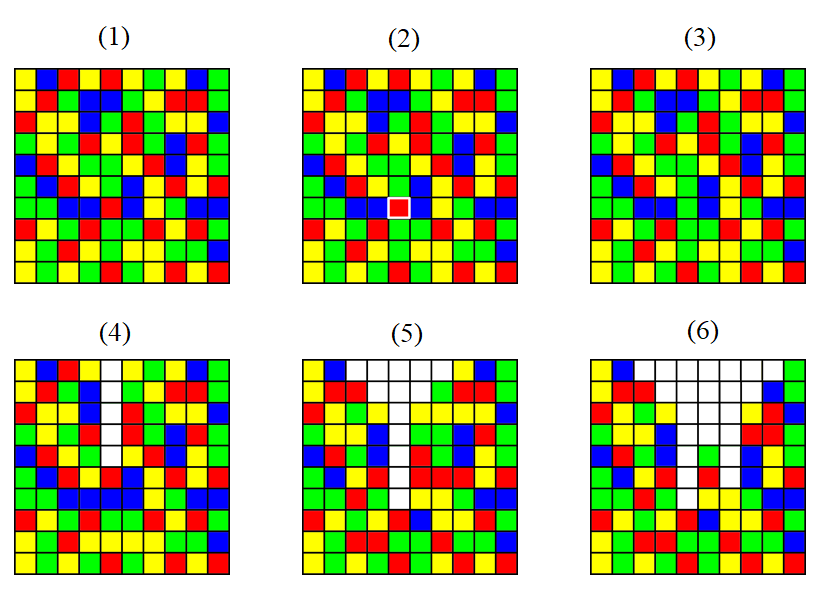
\includegraphics[height=80truemm]{turn}
	\caption{er wordt een blok gekozen om op te drukken, in dit geval een rode blok. De blok verandert met een 1/3 kans in een groene blok. Omdat er meer als 2 blokken van dezeflde kleur op een rij staan worden deze verwijderd en de bovenstaande blokken vallen naar beneden. Dit wordt herhaald tot er niet meer als 2 blokken van dezelfde kleur op een rij staan}
	\label{figure:initialboard}
\end{figure}
\subsection{Strategi\"{e}n}
Ik heb 4 strategiën ontwikkeld om het spel te spelen.
\begin{itemize}
	\item Uniforme strategie
	\item Kleuren ratio strategie
	\item Mogelijke score strategie
	\item Gewogen score strategie
\end{itemize}
Deze strategiën kunnen gebruikt worden om het spel te spelen op een bepaalde wijze. Elke strategie kiest altijd 1 blok uit de mogelijke blokken die beschikbaar zijn. Welk blok dit is hangt van de strategie af.

\subsubsection{Uniforme strategie}
Als de uniforme strategie wordt toegepast is de kans dat een blok gekozen wordt uniform voor elk blok in het spelbord. Voor een 10x10 bord is de kans dat een blok wordt gekozen . In figuur 4 zien we alle mogelijke keuzes die de uniforme strategie kan kiezen in het gegeven bord.
\begin{figure}
	\centering
	\includegraphics[height=70truemm]{uniform\string_strategy}
	\caption{In de uniforme strategie kunnen alle blokken gekozen worden met een uniforme kans verdeling. De kans is 1/100 voor elke blok in dit geval}
	\label{figure:initialboard}
\end{figure}

\subsubsection{Kleuren ratio strategie}
Voor de kleuren ratio strategie worden eerst alle blokken met dezelfde kleur opgeteld. Uit de kleur met het minst aantal blokken wordt uniform een blok gekozen. In figuur 5 zien we dat de blauwe blokken in de minderheid zijn. De strategie zorgt ervoor dat er uniform een blauwe blok wordt gekozen.
\begin{figure}
	\centering
	\includegraphics[height=70truemm]{color\string_ratio\string_strategy}
	\caption{In bovenstaande figuur is de kleuren ratio voor de blauwe blokken het minst. Hier wordt uniform een blauwe blok gekozen met een 1/17 kans voor elke blok}
	\label{figure:initialboard}
\end{figure}

\subsubsection{Mogelijke score strategie}
In de mogelijke score strategie wordt voor elke blok apart nagegaan of deze een mogelijke score kan hebben. Een blok kan een mogelijke score hebben als deze blok kan veranderen in een kleur die een score oplevert. In figuur 6 ziet u alle blokken aangeduid die een mogelijke score kunnen opleveren. Er wordt 1 blok uit deze blokken gekozen met een uniforme kansverdeling.
\begin{figure}
	\centering
	\includegraphics[height=70truemm]{possible\string_score\string_strategy}
	\caption{In een mogelijke score strategie wordt er uniform een blok gekozen uit alle blokken met een mogelijke score. In dit geval zijn er 48 blokken met een mogelijke score dus de kansverdeling is 1/48 voor elke blok}
	\label{figure:initialboard}
\end{figure}
\subsubsection{Gewogen score strategie}
De gewogen score strategie is een uitbreiding op de mogelijke score strategie waar we niet enkel naar de mogelijke score zien, maar naar de gewogen score. Elke blok kan veranderen van kleur aan de hand van een kansverdeling. De gewogen score strategie houdt rekening met deze kansverdeling. De gewogen score wordt berekend aan de hand van de score als een blok in Rood/Groen/Blauw/Geel verandert gewogen met de kans dat de blok verandert in Rood/Groen/Blauw/Geel.

\bibliographystyle{plain}
\bibliography{./biblio}

\newpage
% ----------------------- Achterblad ------------------------------
% Vergeet niet de tekst aan te passen:
% - Afdeling
% - Adres van de afdeling
% - Telefoon en faxnummer
% -----------------------------------------------------------------
\thispagestyle{empty}
\sffamily
%
\begin{textblock}{191}(113,-11)
{\color{blueline}\rule{160pt}{5.5pt}}
\end{textblock}
%
\begin{textblock}{191}(168,-11)
{\color{blueline}\rule{5.5pt}{59pt}}
\end{textblock}
%
\begin{textblock}{183}(-24,-11)
\textblockcolour{}
\flushright
\fontsize{7}{7.5}\selectfont
\textbf{Faculteit Computerwetenschappen}\\
Geel Huis, Kasteelpark Arenberg 11 bus 2100\\
3001 LEUVEN, BELGI\"{E}\\
tel. + 32 16 32 14 01\\
%fax + 32 16 00 00 00\\
www.kuleuven.be\\
\end{textblock}
%
\begin{textblock}{191}(154,-7)
\textblockcolour{}
\includegraphics*[height=16.5truemm]{sedes}
\end{textblock}
%
\begin{textblock}{191}(-20,235)
{\color{bluetitle}\rule{544pt}{55pt}}
\end{textblock}
\end{document}